\documentclass[12pt, oneside]{report}

\usepackage[T1]{fontenc}
\usepackage[utf8]{inputenc}
\usepackage[italian, english]{babel}

\usepackage{microtype}
\usepackage{newpxtext}

\usepackage[subpreambles=true]{standalone}
\usepackage{import}
\usepackage{float}
\usepackage{titling}

\newcommand{\subtitle}[1]{%
  \posttitle{%
    \par\end{center}
    \begin{center}\large#1\end{center}
    \vskip0.5em}%
}

\newcommand\tab[1][1cm]{\hspace*{#1}}

\graphicspath{{./assets/diagrams/}}

\begin{document}

	\title{ER-RM translation with examples}
	\subtitle{Taken form prof. Yannis Velegrakis lectures}
	\author{Conti Samuele \and Daniotti Filippo}
	\date{\today}
	\maketitle

\chapter{Translating ER into RM}
The best way to learn this mechanism is to proceed by examples.\\
Let's start with this classic:

\begin{figure}[H]
	\centering
	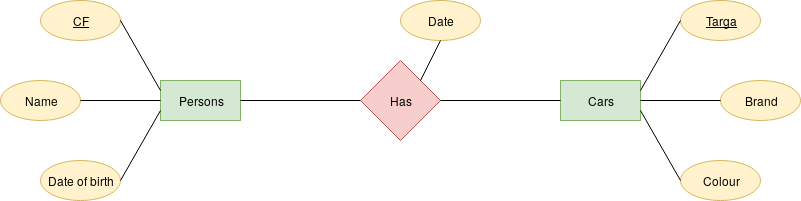
\includegraphics[width=\textwidth,keepaspectratio]{diagram1_00.png}
	\caption{The classic example}
	\label{diagram1_00}
\end{figure}

When we want to translate an Entity Relationship Diagram (ER) into a Relational Model (RM) we have to follow certain rules, let's check them out.

\paragraph*{Rule \#1} Every entity is a table and its attributes are the columns of the table.

\paragraph*{Rule \#2} Each relationship is a table and its attributes are part of the columns of the table; also the Keys of the entities involved in the relation become columns and they are flagged as Foreign Keys (FK). The Key of the table must be composed by the FKs.\\

Let's put this in practice:\\
\bigskip

\noindent \begin{minipage}[t]{0.48\textwidth}
	PERSONS
	\begin{table}[H]
		\centering
		\subimport{assets/tables/}{phc-pers.tex}
	\end{table}
	\texttt{PERSONS(\underline{CF}, Name, Birth date)}
\end{minipage}
\hspace{.04\textwidth}
\begin{minipage}[t]{.48\textwidth}
	CARS
	\begin{table}[H]
		\centering
		\subimport{assets/tables/}{phc-cars}
	\end{table}
	\texttt{CARS(\underline{Targa}, Brand, Color)}
\end{minipage}\\

\bigskip
That was pretty easy, wasn't it? Now it's time to draw the relation table:
\vskip 20pt

\begin{center}
	HAS
	\begin{table}[H]
		\centering
		\subimport{assets/tables/}{phc-has}
	\end{table}
	\texttt{HAS(\underline{CF, Targa}, Date)}
\end{center}

\vskip 20pt
Well, that's clear. Now it's time to mix things up a little bit.
What if a car can't be owned by different people? (see \ref{diagram1_01})
\begin{figure}[H]
	\centering
	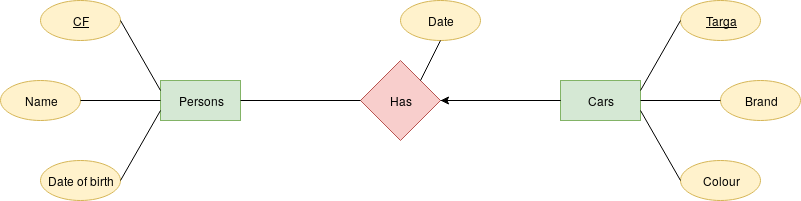
\includegraphics[width=\textwidth,keepaspectratio]{diagram1_01.png}
	\caption{A car now can have at most one owner}
	\label{diagram1_01}
\end{figure}
We must use only \texttt{Targa} as Key in the HAS table. This leads us to the first exception to Rule \#2	:

Each many to one relationship become a relation as in Rule \#2 but the Key is \emph{only} the Key of the 'many' part.

Let's see this rule applied:
\vskip 20pt
\begin{minipage}[c]{0.45\textwidth}
	\begin{center}
		HAS
		\begin{table}[H]
			\centering
			\subimport{assets/tables/}{phc-has_v1}
		\end{table}
	\end{center}
\end{minipage}
\hspace{.05\textwidth}
\begin{minipage}[c]{0.50\textwidth}
	\texttt{HAS(CF, \underline{Targa}, Date)}\\
	\tab[.4cm] \texttt{	CF Foreign Key to PERSONS}\\
	\tab[.4cm] \texttt{	Targa Foreign Key to CARS}
\end{minipage}


\vskip 20pt
And what if we want the car to have also at least one owner? (see \ref{diagram1_02})
\begin{figure}[H]
	\centering
	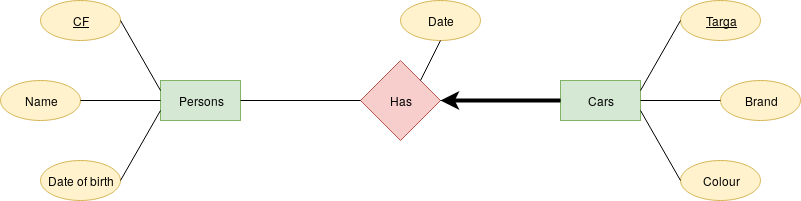
\includegraphics[width=\textwidth,keepaspectratio]{diagram1_02.png}
	\caption{A car now can have at most one owner}
	\label{diagram1_02}
\end{figure}
This way a car must be owned by one (and only one) person, so it makes no sense to keep separately the HAS table and the CARS table, and this leads us to the second exception to Rule \#2:

Each many to one and total partecipation relationship does not become a relation by itself, but its attributes and the Keys of the 'one' entity are added in the attributes of the 'many' entity. The Key of the 'one' entity must be marked as Foreign Key and has to be requested to be \emph{not null}.

Therefore in our case the solution is to delete the HAS table and add two columns to the CARS table, one for \texttt{Date} and one for \texttt{CF}, which will be a FK and will be requested to be \emph{not null}.
That's the representation in RM:
\vskip 20pt
\noindent \begin{minipage}[c]{0.42\textwidth}
	\begin{center}
		CARS
		\begin{table}[H]
			\centering
			\subimport{assets/tables/}{phc-cars_v2}
		\end{table}
	\end{center}
\end{minipage}
\hspace{.01\textwidth}
\begin{minipage}[c]{0.57\textwidth}
	\texttt{CARS(\underline{Targa}, Brand, Color, CF, Date)}\\
	\tab[.4cm] \texttt{	CF not null}\\
	\tab[.4cm] \texttt{	CF Foreign Key to PERSONS}
\end{minipage}
\vskip 20pt

Going back to diagram \ref{diagram1_00}, what if we want to keep in memory all the times someone rent the same car?
Now we cannot do that because, being the Key, \texttt{Targa} cannot appear twice in the table.
The solution here is to use also \texttt{Date} as a Key.
But that's not feasible because, as we stated in Rule \#2, only Keys of the entities are used as Key in the relation table, and \texttt{Date} is not an entity; hence we have to redesign our diagram as this:
\begin{figure}[H]
	\centering
	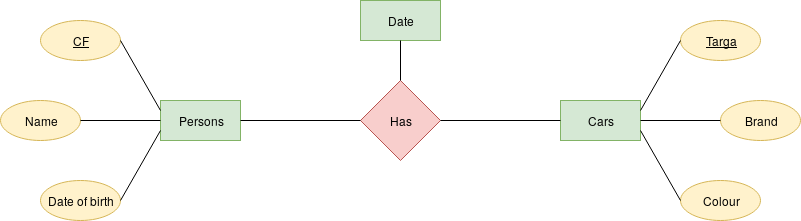
\includegraphics[width=\textwidth,keepaspectratio]{diagram1_03.png}
	\caption{Now Date is an entity}
	\label{diagram1_03}
\end{figure}
\vskip 20pt

Now we want every rent to have an insurance, so we have to create a new entity called INSURANCES and link it to the RENT relation as this:
\begin{figure}[H]
	\centering
	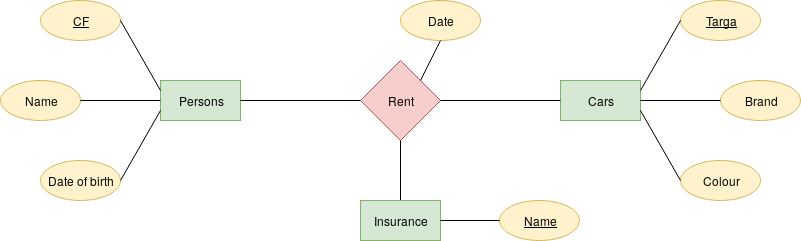
\includegraphics[width=\textwidth,keepaspectratio]{diagram1_04.png}
	\caption{We added INSURANCES as an entity}
	\label{diagram1_04}
\end{figure}
\hspace{0.25\textwidth}
\begin{minipage}{0.5\textwidth}
	\texttt{RENT(\underline{Owner, Car, Name}, date)}\\
		\tab[.8cm] \texttt{Owner FK to PERSONS}\\
		\tab[.8cm] \texttt{Car FK to CARS}\\
		\tab[.8cm] \texttt{Name FK to INSURANCES}
\end{minipage}
\vskip 20pt

And now we decide that the insurance is no more necessary for a rent, how do we set it as a field that can be \emph{null}?
We have to link it to RENT with a relationship.
But we can't link two relationships together: we must aggregate PERSONS, RENT and CARS so that we can treat this set as an entity and then we can link to the aggregated entity the INSURANCES with another relationship (see \ref{diagram1_05}).
\begin{figure}[H]
	\centering
	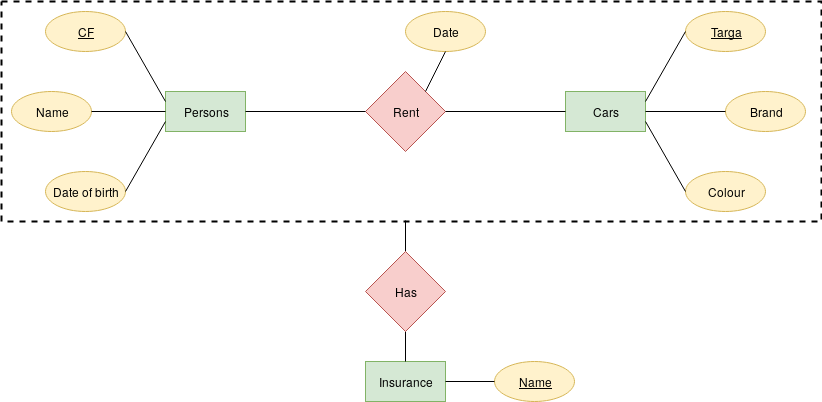
\includegraphics[width=\textwidth,keepaspectratio]{diagram1_05.png}
	\caption{Now PERSONS, RENT and CARS are aggregated}
	\label{diagram1_05}
\end{figure}
In this case what's going to be the Key of RENT?
\vskip 10pt
\texttt{RENT(\underline{Owner, Car}, date)}\\
	\tab[.8cm] \texttt{Owner FK to PERSONS}\\
	\tab[.8cm] \texttt{Car FK to CARS}
\vskip 10pt
\noindent And which should be the Key of HAS?\\
Keeping in mind Rule \#2 we have that the Keys of a relationship must be the Keys of the entities involved, marked as Foreign Key, therefore:
\vskip 10pt
\texttt{HAS(\underline{Owner, Car, Name})}\\
	\tab[.8cm] \texttt{(Owner, Car) FK to RENT}\\
	\tab[.8cm] \texttt{Name FK to INSURANCE}
\vskip 10pt
And now the last question about this example: what's the difference between \ref{diagram1_04} and \ref{diagram1_06}?
\begin{figure}[H]
	\centering
	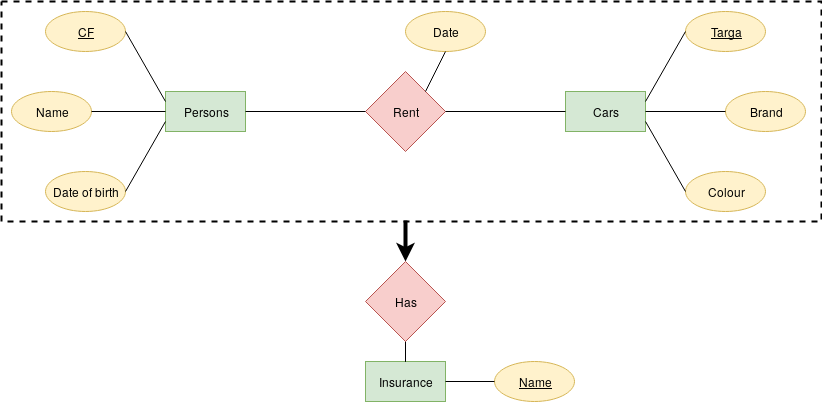
\includegraphics[width=\textwidth,keepaspectratio]{diagram1_06.png}
	\caption{Note the particular form of the diagram}
	\label{diagram1_06}
\end{figure}
The difference is:
\begin{itemize}
	\item In \ref{diagram1_04} you \emph{must} use \texttt{Name} as Key in the RENT table, because INSURANCES is an entity involved in RENT relation (Rule \#2); therefore a person can rent the same car multiple times given that he or she uses a different insurance.\\
	\item In \ref{diagram1_06} you don't have to use \texttt{Name} as Key in the RENT table, therefore it is not possible for a person to rent the same car with two different insurances (even if the insurance changes the Key remains the same).
\end{itemize}

\section{Let's talk about inheritance}
Now it's time to see a little bit of inheritance, as before we're starting with an example:
\begin{figure}[H]
	\centering
	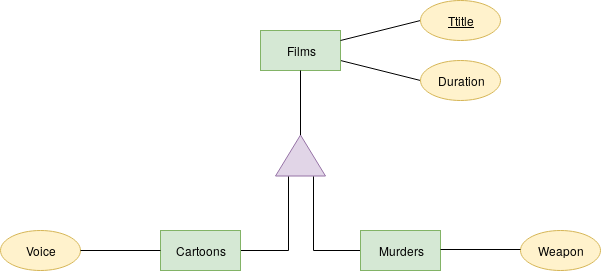
\includegraphics[width=\textwidth,keepaspectratio]{diagram2_00.png}
	\caption{An example of inheritance}
	\label{diagram2_00}
\end{figure}
There are three ways to translate ER inheritance into RM:
\begin{enumerate}
	\item The first approach is to have a different table for every entity, the tables of the children entities will contain also the attributes inherited by the parent entity.
	\vskip 5pt
	\texttt{FILMS(\underline{Title}, Duration)}\\
	\texttt{CARTOONS(\underline{Title}, Duration, Voice)}\\
	  	\tab[.8cm] \texttt{Title FK to FILMS}\\
	\texttt{MURDER(\underline{Title}, Duration, Weapon)}\\
		\tab[.8cm] \texttt{Title FK to FILMS}
	\vskip 5pt
	The bad aspect of this technique is that we store the different entity-types in different places, for instance Shrek is stored into CARTOONS table, therefore if we want to query the database by \texttt{Title} and ask for Shrek we have to navigate through all the tables. Also if we want to query how many films the database contains we will have to search in all the tables.
	\item The second approach is to have a different table for every entity, but the tables of the children entities contain only their specific attributes and the Key attribute of the parent entity, which will be also the child entity's Key (and Foreign Key).
	\vskip 5pt
	\texttt{FILMS(\underline{Title}, Duration)}\\
	\texttt{CARTOONS(\underline{Title}, Voice)}\\
	  	\tab[.8cm] Title FK to FILMS\\
	\texttt{MURDER(\underline{Title}, Weapon)}\\
		\tab[.8cm] \texttt{Title FK to FILMS}
	\vskip 5pt
	This strategy is better because all the entities are stored in the FILMS table and therefore if we're querying, for instance, \texttt{Title} or \texttt{Duration}, we have to look only into the FILMS table. The films that are cartoons - like Shrek - are going to be registered also in the CARTOONS table, and there we will find their \texttt{Voice} attribute.
	The downside of this approach is that when we query, let's say, \texttt{Duration} and \texttt{Voice} we have to look into two different tables at the same time, and that's actually more complicated than we need.
	\item The third approach is to store all the films in the same table with all the possible attributes of the parent entity and the children entities, which will be filled with a \emph{null} value if the film stored isn't a cartoon or a murder.
	\vskip 5pt
	\texttt{FILMS(\underline{Title}, Duration, Voice, Weapon)}\\
	\tab[.4cm] \texttt{Duration is not-null}\\
	\tab[.4cm] \texttt{Voice and Weapon can be null}
	\vskip 5pt
	Thinking in a querying way that's the best approach, for every research in the database you have to navigate only through a table. Anyway in the real life, where problems are way much complex than our examples, this technique can become tricky too.
\end{enumerate}

\section{Weak Entities}
Now let's take a quick look at the translation of Weak Entities, i.e. entities that cannot exist on their own.\\
\begin{figure}[H]
	\centering
	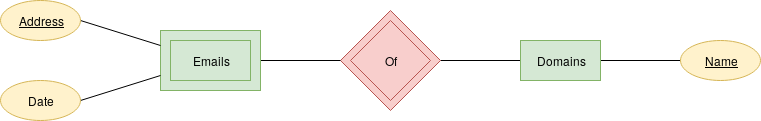
\includegraphics[width=0.8\textwidth,keepaspectratio]{diagram4_00.png}
	\caption{E-mail cannot exist if domain doesn't}
	\label{diagram4_00}
\end{figure}
\vskip 5pt
The translation is simple: DOMAINS is a straight entity, so we list all its attributes and underline the Key, and then we do the same for E-MAILS, and its Composite Key is going to be its Key (\texttt{Address}) plus the Key of its straight entity (\texttt{Name}, in this case), which is also a Foreign Key.\\\\
\texttt{DOMAINS(\underline{name})}\\
\texttt{EMAILS(\underline{address}, date, \underline{name})}\\
\tab[.4cm] \texttt{name Foreign Key to DOMAINS}
\vskip 5pt

\chapter{Reverse engineering: from RM to ER}
Sometimes you may want to translate an RM back to its ER model, so here we provide some examples and basic rules in order to get it done.

For instance, let's consider the following statements:\\\\
\texttt{A(\underline{x}, y)}\\
\texttt{B(\underline{u}, \underline{v})}\\
\tab[.4cm] \texttt{v Foreign Key to A}\\
\tab[.4cm] \texttt{u Foreign Key to C}\\
\texttt{C(\underline{m}, n)}
\vskip 5pt
B has two Foreign Keys, one points to A and the other one points to C, so B is a relationship between A and C.
\begin{figure}[H]
	\centering
	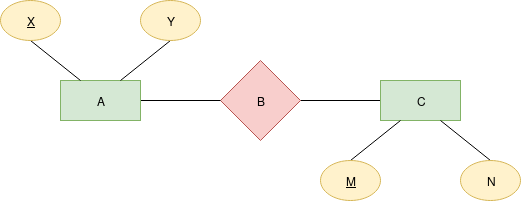
\includegraphics[width=0.8\textwidth,keepaspectratio]{diagram3_00.png}
	\caption{Justa figure}
	\label{diagram3_00}
\end{figure}
\vskip 5pt
But now we change it up just a little, and we want something like this:\\\\
\texttt{A(\underline{x}, y)}\\
\texttt{B(\underline{u}, v)}\\
\tab[.4cm] \texttt{v Foreign Key to A}\\
\tab[.4cm] \texttt{u Foreign Key to C}\\
\texttt{C(\underline{m}, n)}
\vskip 5pt
It looks similar, but it's not the same: \texttt{v} is not a Key of B anymore, so we can have multiple \texttt{v}s for just one \texttt{u}, so the relationship from C to A has become a many to one relationship.
\begin{figure}[H]
	\centering
	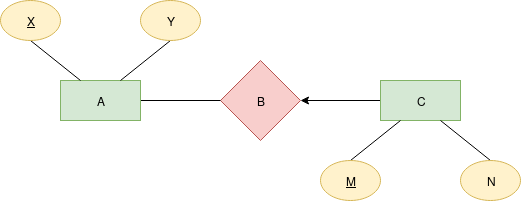
\includegraphics[width=0.8\textwidth,keepaspectratio]{diagram3_01.png}
	\caption{Justa nother figure}
	\label{diagram3_01}
\end{figure}
\vskip 5pt
Here it is another example:\\\\
\texttt{C(\underline{m}, n, v)}\\
\tab[.4cm] \texttt{m Foreign Key to A}\\
\texttt{A(\underline{x}, y)}\\
\vskip 5pt
This is a IS-A and C is child to A, because the Foreign Key \texttt{m} is also the only Key of C.

\section{Advanced examples}
Let's take a look at a few more examples:
\subsection*{Esempio A}
\texttt{Person(\underline{cf}, pname, paddress)}\\
\texttt{Car(\underline{cid}, targa)}\\
\texttt{Insurance(\underline{iid}, iname)}\\
\texttt{Has(\underline{cf, cif})}\\
\tab[.4cm] \texttt{cf FK to Person}\\
\tab[.4cm] \texttt{cif FK to Car}\\
\texttt{Has2(\underline{cf, cif, iid})}\\
\tab[.4cm] \texttt{(cf, cif) FK to Has}\\
\tab[.4cm] \texttt{iid FK to Insurance}
\vskip 8pt
As for the previous examples in this RM are present two relations, which are HAS and HAS2, we can say that these are relations because they have two Foreign Keys to other elements; the elements without FKs must be entities, so we have PERSONS, CARS and INSURANCES as entities.
The intresting detail in this case is that HAS2 has this FK: '\texttt{(cf, cif) FK to Has}'.\\
We know that it's impossible to have a relation linked to another, therefore it's impossible to have a link between HAS and HAS2; this implies that there is an aggregation between PERSONS, CARS and HAS.\\
Let's see what I'm babbling about:
\begin{figure}[H]
	\centering
	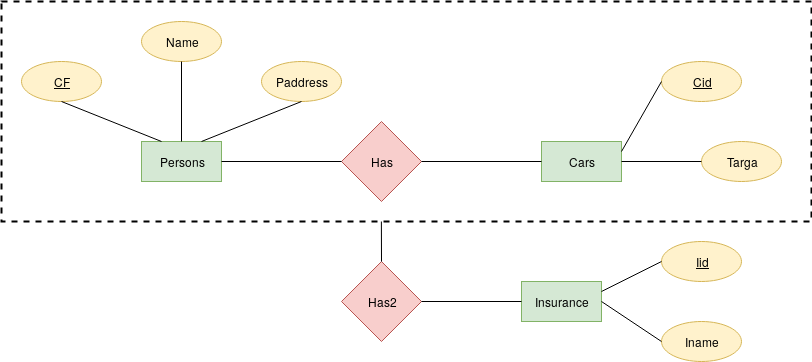
\includegraphics[width=0.8\textwidth,keepaspectratio]{diagram6_00.png}
	\label{diagram6_00}
\end{figure}

\subsection*{Esempio B}
\texttt{Person(\underline{cf}, pname, paddress)}\\
\texttt{Student(\underline{mat}, corso)}\\
\tab[.4cm] \texttt{mat FK to Person}
\vskip 8pt
In this case the peculiarity is that the element STUDENT has \texttt{mat} as only Key, and it's also a FK to PERSON, this means that there must be an IS-A between the two entities; let's check the ERD:

\begin{figure}[H]
	\centering
	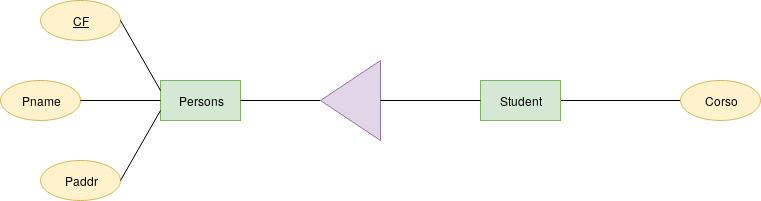
\includegraphics[width=0.8\textwidth,keepaspectratio]{diagram6_01.png}
	\label{diagram6_01}
\end{figure}

\subsection*{Esempio C}
\texttt{Person(\underline{cf}, pname, paddress)}\\
\texttt{Student(\underline{mat}, pers, corso)}\\
\tab[.4cm] \texttt{pers FK to Person}
\vskip 8pt
This example is slightly different from the previous one, but its meaning is opposite. We see that STUNDENT has \texttt{mat} as Key but it is no more an FK to PERSON, nontheless there's a new attribute in STUDENT which is an FK to PERSON: that's \texttt{pers}.\\
This means that a relation is involved, and this relation has a precise form: it is a many to one, in fact a STUDENT can be linked only to one (at most one) PERSON; in contrast we don't have any limitation for the PERSON side of the relation.

\begin{figure}[H]
	\centering
	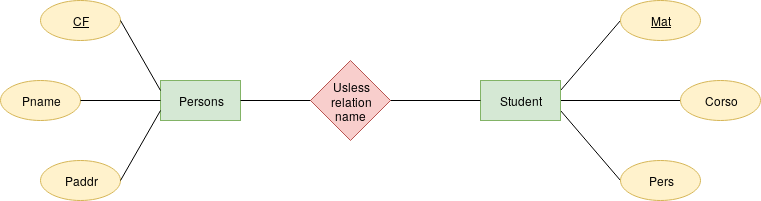
\includegraphics[width=0.8\textwidth,keepaspectratio]{diagram6_02.png}
	\label{diagram6_02}
\end{figure}

\subsection*{Esempio D}
\texttt{Person(\underline{cf}, pname, paddress)}\\
\texttt{Student(\underline{mat, pers}, corso)}\\
\tab[.4cm] \texttt{pers FK to Person}
\vskip 8pt
In this last case we see that the Key of STUDENT is composed by \texttt{mat} and \texttt{pers}, which is still a FK to PERSON.\\
The fact that the Key of STUDENT is in part composed by a FK means that STUDENT is a Weak Entity; therefore the ERD is the following one:

\begin{figure}[H]
	\centering
	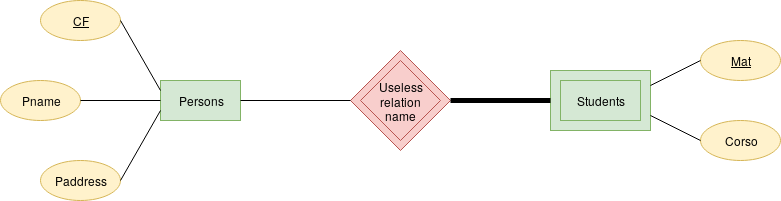
\includegraphics[width=0.8\textwidth,keepaspectratio]{diagram6_03.png}
	\label{diagram6_03}
\end{figure}

\section{Summing it up}
Now let's point out four basic rules if you are into troubles with reverse engineering and you want to have it done quickly:
\paragraph{Rule \#1} If there are two or more Foreign Keys wich are the components of the Key, that's a many to many relationship.
\paragraph{Rule \#2} If there's a Foreign Key which is not a part of the Key, what we have is a many to one relationship.
\paragraph{Rule \#3} If there is a Foreign Key which is the only Key of that table, what we have is an IS-A.
\paragraph{Rule \#4} If there is a Foreign Key which is a part of the Key but it's NOT the whole Key of that table, what we have is a Weak Entity relationship.

\end{document}
